%%%%% ------------------------------------------------------------------------------------------
%%
%%                               Document Template
%%
%%  Project Name: njustThesis
%%  Repository: https://github.com/packyan/NJUST_Master_Thesis_Latex_Template
% 	From :https://github.com/jiec827/njustThesis
%%
%%%%% ------------------------------------------------------------------------------------------
%% re-written by Dengan <packyande@gmail.com>
%% Last-modified: 2020-08-20
%%
%% This program can be redistributed and/or modified under the terms
%% of the GNU Public License, version 2.
%%%%% ------------------------------------------------------------------------------------------
%%
%%%%*************************Document Class Declaration*******************************
%%

\documentclass[UTF8,AutoFakeBold]{sty/njustThesis}% thesis template of the Nanjing Univ of Sci & Tech
%% Options:
%% [draftinfo] % show draft version information
%%%%% --------------------------------------------------------------------------------
%%
%%%%**************************Command Define and Settings***************************
%%
%目录 chapter 行距

\usepackage{cite}
\usepackage[njust]{sty/commons}% common settings
\usepackage{sty/custom}% user defined commands
%\usepackage[numerical]{bib/gbt7714}
%%%%% ------------------------------------------------------------------------------------------
%%%%*********************************Content**********************************************
%%
% setting times new roman
%\usepackage[T1]{fontenc}
%\usepackage{mathptmx}
\usepackage{fontspec}
\setmainfont{Times New Roman}
%\usepackage{tocloft}

\usepackage{etoolbox}

\makeatletter
\pretocmd{\chapter}{\addtocontents{toc}{\protect\addvspace{-15\p@}}}{}{}
%\pretocmd{\section}{\addtocontents{toc}{\protect\addvspace{5\p@}}}{}{}
\makeatother


\begin{document}

%%
%%%%% ------------------------------------------------------------------------------------------
%%
%%%%*********************************Frontmatter******************************************
%%
%% Frontmatter of Title page, Table of contents, Preface chapter.
%%
%% >>> Cover
%%
%
%%% >>> Title Page
%%
%%
%%%%********************** Chinese Title Page ****************************************
%%
  \classification{}
  \confidential{}
  \UDC{}
%% 标题格式 \title[short title for headers]{Long title of thesis}
  \title[基于某某的某技术研究]{基于某某的某技术研究}
  \titleUpp{基于某某的某技术研究}
  \titleLow{}
  %\xeCJKsetup{AutoFakeBold=true,AutoFakeSlant=true}
  \author{李四四}
  \advisor{王五五}
  \advisortitle{教授}
  \degree{某学硕士}
  \major{{控制理论与控制工程}}
  \interest{{计算机图形学}}
  \school{南京理工大学}
  \submitdate{2020年12月}
  \incoverdate{2021年3月}
  %
 % \titleBackbone{南\\京\\理\\工\\大\\学\\硕\\士\\学\\位\\论\\文\\模\\板}
 % \schoolBackbone{南\\京\\理\\工\\大\\学}
 
 \titleBackbone{ }%\\ \\ \\ \\ \\ \\ \\ \\ \\ \\ \\ \\ \\}
 \schoolBackbone{ }% \\ \\ \\ \\ \\ }
%%
%%%%********************** English Title Page ****************************************
%%
  \englishtitle{Dissertation template of Nanjing University of Science and Technology}
  \englishauthor{Sisi Li}
  \englishadvisor{Wuwu Wang}
  \englishinstitute{Nanjing University of Science \& Technology}
  \englishdate{December, 2020}
  \englishdegree{Dissertation}
%%
%%%%********************** Generate CHN & Eng Title ***********************************
%%%
%%
\maketitle
%%
\makeincovertitle
%%
\makeenglishtitle
%% make statement page
\makeatletter
\cleardoublepage
\thispagestyle{empty}
\begin{center}
\statement{
本学位论文是我在导师的指导下取得的研究成果,尽我所知,在本学位论文中,除了加以标注和致谢的部分外,不包含其他人已经发表或公布过的研究成果,也不包含我为获得任何教育机构的学位或学历而使用过的材料。与我一同工作的同事对本学位论文做出的贡献均已在论文中作了明确的说明。
}%

\accredit{
南京理工大学有权保存本学位论文的电子和纸质文档,可以借阅或上网公布本学位论文的部分或全部内容,可以向有关部门或机构送交并授权其保存、 借阅或上网公布本学位论文的部分或全部内容。对于保密论文,按保密的有关规定和程序处理。
}
\end{center}
\clearpage
\if@twoside
  \thispagestyle{empty}
  \cleardoublepage
\fi
 \makeatother
%%%%*********************************** END *******************************************

%%
%% >>> start frontmatter page No.
%%
\frontmatter
%%
%% >>> Abstract
%%
\begin{abstract}

简单介绍论文所研究的问题以及创新点。

\keywords{}
\end{abstract}


\begin{englishabstract}
English translation.

\englishkeywords{}
\end{englishabstract}
%%
%%% >>> List of Content
%%
%\clearpage

%%修改点密度
%\makeatletter
%%\renewcommand*\l@chapter{\@dottedtocline{1}{0em}{0.0em}}
%\renewcommand*\l@section{\@dottedtocline{1}{24pt}{34pt}}
%\renewcommand*\l@subsection{\@dottedtocline{2}{23pt}{23pt}}
%%\renewcommand*\l@subsubsection{\@dottedtocline{3}{36pt}{36pt}}
%%\renewcommand*\l@paragraph{\@dottedtocline{4}{48pt}{48pt}}
%%\renewcommand*\l@subparagraph{\@dottedtocline{5}{60pt}{60pt}}
%\makeatother
%

\makeatletter
\def\@dotsep{1}%就在这儿改,把2改成其他什么,默认是4.5,就是点之间距离为4.5mu
\makeatother
%这里使用tocloft包提供的命令:\cftbeforeXskip 这里的X可以用chap, sec等来替代,表示章,节的上部距离。 如

{
  \hypersetup{linkcolor=black}
  \tableofcontents% contents catalog
}



%\phantomsection
%\addcontentsline{toc}{chapter}{目\NJUSTspace 录}
% 目录是否参与编号

%% list figures and tables sperately
%\listoffigures%   figures catalog
%\addcontentsline{toc}{chapter}{插图目录}
%\listoftables%    tables catalog
%\addcontentsline{toc}{chapter}{表格目录}
% list figures and tables together
%\listoffiguresandtables
%\addcontentsline{toc}{chapter}{图表目录}
%%
% {\centering\printnomenclature}% nomenclature catalog
% \addcontentsline{toc}{chapter}{术语表}
%%
%%%%% ------------------------------------------------------------------------------------------
%%
%%%%*********************************Mainmatter******************************************
%%
%% Main topics.
\mainmatter
%%
%%% >>> Main Contents
%%

\chapter{绪论}
\label{chap:introduction}

\section{研究背景和意义}
点云(Point Cloud)是一种高效的三维对象表达方式。点云是由一组点构成的集合,每个点由其三维坐标$(x,y,z)$和可能的其他属性(如颜色信息或者法线方向)组成。
%由于点云能够高效地表示三维空间中的任意形状,所以点云被广泛应用于各个领域。同时,随着深度传感器技术的发展,例如微软的Kinect深度相机、LiDAR 三维扫描仪、光场相机、智能手机搭载的结构光传感器等能够方便地采集三维点云数据,点云数据的应用前景巨大。但同时缺少高效、灵活的点云处理技术,因此,越来越多的点云数据亟待被识别加以利用,将点云处理的结果应用于各种实际应用场景中去,点云识别技术成为了一个具有巨大研究价值和应用前景的学科方向,例如点云的分类、分割技术等是目前活跃的研究课题。点云数据一般被认为是非欧氏数据(Non-Euclidean data)。传统的深度学习技术大多数基于结构化数据,故大多数先前的利用卷积神经网络来对点云进行识别的工作,多将点云数据转化为多视角的二维图像或对点云进行体素化,把点云数据转化为某种规则的结构化数据,再输入网络进行学习。然而,对点云进行这样的转化会产生大量的临时数据并会引入量化误差,所以如让神经网络处理原始点云数据成为了一个研究热点。相较于具有网格结构的欧式数据,点云具有旋转不变性、尺度不变性、顺序不变性、平移不变性等特点\cite{wang2019dynamic},标准卷积网络无法克服这些问题,所以如何解决点云数据存在的这些问题,成为了将深度学习技术应用于点云识别的一大障碍,同时也是目前几何深度学习(Geometric Learning)的研究热点。
公式测试:
\begin{equation}
	h^{l+1} = \sum_i {e_i - e_j}
\end{equation}

\begin{equation}
	max\sum_{i \in \Omega_t^{load} }\sum_{j \in \Omega_t^{FD} }w_{ij,t}x_{ij,t}P_{ij,t}^{La}
\end{equation}

内联公式测试$N_i = \{  N_{ij}^{P}\}$

\subsection{}
%\begin{figure}[htbp]
%\centering
%\subfigure[心脏电影(一帧)]{
%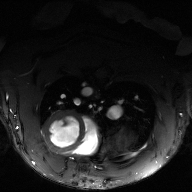
\includegraphics[width=2.11in]{img/intro/cine.png}
%}
%\subfigure[胸部DCE-MRI(一帧)]{
%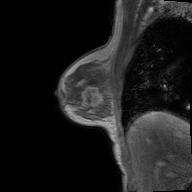
\includegraphics[width=2.11in]{img/intro/breast.png}
%}
%\subfigure[心脏灌注(一帧)]{
%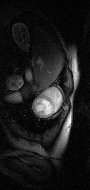
\includegraphics[width=1in]{img/intro/perfusion.png}
%}
%\centering
%\caption{动态MR图像举例。}
%\label{fig:dynamic}
%\end{figure}

\section{本文的主要研究内容和章节安排}

针对xxx存在的问题,本文提出xxx。

第二章 ...

第三章 ...

第四章 ...

第五章,我们对本文的工作进行了总结并给出了下一步工作展望。





%


\chapter{第二章}
\label{chap:chap2}

\section{模型的提出}
\section{模型的离散化和算法}
\section{数值实验数据与评价方法}
\section{数值实验结果}
\section{本章小结}

















%
\chapter{第三章}
\label{chap:chap3}



%
\chapter{基于xxx的xxxx实现}
\label{chap:chap4}
模式识别是将采集到的指纹数据和字典进行匹配,Ma等\cite{mrf}使用了模板匹配的方法来进行参数图的重建。记$X=\{x_n\in \mathbb{C}^L\}, n=1,...,N$为采集到的指纹数据,$\mathcal{D}=\{d_k\in \mathbb{C}^L\},k=1,...,K$为生成的字典。那么模板匹配即为从从字典$\mathcal{D}$中选取和$x_n$内积最大的元素:
	\begin{equation}
	\hat{k}_n = \argmax_k \left|\left\langle \mathbf{d}_k,\mathbf{x}_n \right\rangle \right|.
	\end{equation}
并且质子密度也可以同时计算:
	\begin{equation}
	\hat{\rho}_n=\left|\langle \mathbf{d}_{\hat{k}_n},\mathbf{x}_n \rangle\right|.
	\end{equation}

\begin{algorithm}
	\caption{snapMRF生成字典与匹配详细流程。}
	\label{alg:snapMRF}
	\begin{algorithmic}
		\INDSTATE[-1.25] \textbf{输入:}\texttt{*d\_mrf},\texttt{*d\_params},\texttt{*d\_img}
		\INDSTATE[-1.25] \textbf{输出:}\texttt{*d\_atoms},\texttt{*d\_maps}
		\STATE 01:从CSV文件中读取MRF序列信息,存入\texttt{*d\_mrf};
		\STATE 02:从命令行输入字典参数信息,存入\texttt{*d\_params};
		\STATE 03:初始化状态矩阵\texttt{*d\_w};
		\STATE 04:\textbf{迭代}:从第1个时刻到第$L$个时刻,并行计算所有体素的信号
		\STATE 05:\qquad 使用函数\texttt{fill\_transition\_matrix()}构造转移矩阵$T$;
		\STATE 06:\qquad 使用函数\texttt{apply\_rf\_pulse()}将射频场作用在\texttt{*d\_w}上;
		\STATE 07:\qquad 使用函数\texttt{decay\_signal()}将$T_1$和$T_2$衰减作用在\texttt{*d\_w}上;
		\STATE 08:\qquad 使用函数\texttt{save\_atoms()}将原子的信号保存在\texttt{*d\_atoms}中;
		\STATE 09:\qquad 使用函数\texttt{dephase\_gradients()}将梯度场作用在\texttt{*d\_w}上;
		\STATE 10:\qquad 使用函数\texttt{decay\_signal()}将$T_1$和$T_2$衰减作用在\texttt{*d\_w}上;
		\STATE 11:\textbf{终止迭代};
		\STATE 12:释放\texttt{*d\_w};
		\STATE 13:从RawArray文件中读取指纹数据,存入\texttt{*d\_img};
		\STATE 14:计算剩余显存大小,并根据剩余显存,将\texttt{*d\_img}分为$G$组;
		\STATE 15:\textbf{迭代}:从第1组到第$G$组,在每一组内并行计算所有体素的参数
		\STATE 16:\qquad 使用函数\texttt{MRF\_minimatch()}进行匹配;
		\STATE 17:\qquad 使用函数\texttt{generate\_maps()}生成参数图;
		\STATE 18:\textbf{终止迭代};
		\STATE 19:将\texttt{*d\_atoms}和\texttt{*d\_maps}保存为RawArray文件;
		\STATE 20:释放所有显存和内存。
	\end{algorithmic}
\end{algorithm}

\newpage
翻页测试,左上角章节。





%
\chapter{总结与展望}
\label{chap:future}

参考了\cite{lustig2006}
\section{本文工作总结}
\section{下一步工作展望}


\begin{thanks}
谢谢老板
值此论文完成之际,谨在此向多年来给予我关心和帮助的老师、同学、朋友和家人表示衷心的感谢!

首先,我要感谢我的导师***教授,感谢杨老师在我读博期间给予我的无私帮助和关怀。是他把我领入了图像处理中的数学问题这一领域,本论文的选题、攻关到最终完成,都凝聚着老师的心血,浸透着老师的汗水,他孜孜不倦的工作热情是我学习的榜样。杨老师工作繁忙,但每周都会安排讨论班,不仅拓展了我们的研究广度,还创造了良好的学术氛围。杨老师不仅知识渊博,高瞻远瞩,治学严谨,而且平易近人,品德谦逊,让我受益匪浅,终生难忘,从他身上我学会了许多做学问和为人处世的道理,这将激励我不断追求更高的目标。这里再次向杨老师表示衷心的感谢,师生情谊,难忘终生。

感谢教研室和我一起学习的同学们:**等陪我度过了快乐的博士生涯,给我留下了美好的回忆,使我在紧张的学习之余有了丰富的课余生活,也感谢他们在学习和生活上给予的帮助。

我要深深地感谢我的父母和家人,感谢他们这么多年的理解与支持,感谢他们一直默默地关心我、帮助我,正是他们始终如一的奉献,才使我顺利地完成了学业。在今后的科研工作中,我必会更加努力,来回报你们对我的爱。

最后,再次感谢所有帮助过我的老师和朋友。
\end{thanks}

%%%%% ------------------------------------------------------------------------------------------
%%
%%%%*********************************Appendix********************************************
%%
%% Some subordinate chapters.
%\input{tex/appendix}%
%%%%% ------------------------------------------------------------------------------------------
%%
%%%%********************************Backmatter*******************************************
%%
%% Matters of Bibliography, Glossary, Index.
\backmatter
%%
%%% >>> Acknowledgements
%%
%%
%%% >>> Bibliography
%%
%\bibliographystyle{GBT7714-2005}
%\bibliographystyle{NJUST_GBT7714-2005NLang_Upp}

%
%%
%%% >>> Publications
%%
%\clearpage


\cleardoublepage
\phantomsection
\addtocontents{toc}{\vspace{-15pt}}
\addcontentsline{toc}{chapter}{参考文献} %向目录中添加条目,以章的名义
{\centering  \bibliography{bib/myThesisRefs.bib} }

\begin{publications}{99}
\item[] {\songti\zihao{4}\bf{攻读硕士学位期间已发表的论文:}}
\item 某篇论文[J]
\item 某篇会议

\vspace{1.0cm}
\item[] {\songti\zihao{4}\bf{攻读硕士学位期间参加的科学研究情况:}}
\setcounter{enumiv}{0}
\item 参与xxx
\item 参加xxx

\end{publications}

%%
%%% >>> Resume
%%
%%
\end{document}
%%%%% ------------------------------------------------------------------------------------------
